\documentclass[12pt, a4paper, twoside]{article}
\usepackage{header_tp}
%\includeonly{ej1}
\begin{document}

% -- Carátula --
\newpage{\pagestyle{empty}% **************************************************************************
%
%  Package 'caratula', version 0.3 (para componer caratulas de TPs del DC).
%
%  CON MINIMAS MODIFICACIONES DEL TEAM ORGA2
%
%  En caso de dudas, problemas o sugerencias sobre este package escribir a
%  Brian J. Cardiff (bcardif arroba gmail.com).
%  Nico Rosner (nrosner arroba dc.uba.ar).
%
% **************************************************************************

% ----- Informacion sobre el package para el sistema -----------------------

\NeedsTeXFormat{LaTeX2e}
\ProvidesPackage{caratula}[2005/08/09 v0.3 Para componer caratulas de TPs del DC]
%\usepackage[pdftex]{graphicx}

% ----- Imprimir un mensajito al procesar un .tex que use este package -----

\typeout{Cargando package 'caratula' v0.3 (2005/08/09)}

% ----- Algunas variables --------------------------------------------------

\let\Materia\relax
\let\Submateria\relax
\let\Titulo\relax
\let\Subtitulo\relax
\let\Grupo\relax
\let\Fecha\relax
\let\Logoimagefile\relax

% ----- Comandos para que el usuario defina las variables ------------------

\def\materia#1{\def\Materia{#1}}
\def\submateria#1{\def\Submateria{#1}}
\def\titulo#1{\def\Titulo{#1}}
\def\subtitulo#1{\def\Subtitulo{#1}}
\def\grupo#1{\def\Grupo{#1}}
\def\fecha#1{\def\Fecha{#1}}
\def\logoimagefile#1{\def\Logoimagefile{#1}}

% ----- Token list para los integrantes ------------------------------------

\newtoks\intlist\intlist={}

% ----- Comando para que el usuario agregue integrantes --------------------

\def\integrante#1#2#3{\intlist=\expandafter{\the\intlist
    \rule{0pt}{1.2em}#1&#2&\tt #3\\[0.2em]}}

% ----- Macro para generar la tabla de integrantes -------------------------

\def\tablaints{%
    \begin{tabular}[t]{| l @{\hspace{4ex}} c @{\hspace{4ex}} l|}
        \hline
        \multicolumn{1}{|c}{\rule{0pt}{1.2em} Integrante} & LU &  \multicolumn{1}{c|}{Correo electr\'onico} \\[0.2em]
        \hline \hline
        \the\intlist
        \hline
    \end{tabular}}

% ----- Codigo para manejo de errores --------------------------------------

\def\se{\let\ifsetuperror\iftrue}
\def\ifsetuperror{%
    \let\ifsetuperror\iffalse
    \ifx\Materia\relax\se\errhelp={Te olvidaste de proveer una \materia{}.}\fi
    \ifx\Titulo\relax\se\errhelp={Te olvidaste de proveer un \titulo{}.}\fi
    \edef\mlist{\the\intlist}\ifx\mlist\empty\se%
    \errhelp={Tenes que proveer al menos un \integrante{nombre}{lu}{email}.}\fi
    \expandafter\ifsetuperror}


% ----- \maketitletxt correspondiente a la versión v0.2 (texto) ---------

\def\maketitletxt{%
    \ifsetuperror\errmessage{Faltan datos de la caratula! Ingresar 'h' para mas informacion.}\fi
    \thispagestyle{empty}
    \begin{center}
    \vspace*{\stretch{2}}
    {\LARGE\textbf{\Materia}}\\[1em]
    \ifx\Submateria\relax\else{\Large \Submateria}\\[0.5em]\fi
    \par\vspace{\stretch{1}}
    {\large Departamento de Computaci\'on}\\[0.5em]
    {\large Facultad de Ciencias Exactas y Naturales}\\[0.5em]
    {\large Universidad de Buenos Aires}
    \par\vspace{\stretch{3}}
    {\Large \textbf{\Titulo}}\\[0.8em]
    {\Large \Subtitulo}
    \par\vspace{\stretch{3}}
    \ifx\Grupo\relax\else\textbf{\Grupo}\par\bigskip\fi
    \tablaints
    \end{center}
    \vspace*{\stretch{3}}
    \newpage}

% ----- \maketitle correspondiente a la versión v0.3 (gráfica) -------------

\def\maketitlegraf{%
    \ifsetuperror\errmessage{Faltan datos de la caratula! Ingresar 'h' para mas informacion.}\fi
%
    \thispagestyle{empty}

    \ifx\Logoimagefile\relax\else\includegraphics{\Logoimagefile}\fi\hfill 
\includegraphics{imagenes/logodc.jpg}

    \vspace*{.12 \textheight}

    \noindent \textbf{\huge \Titulo}  \medskip \\
    \ifx\Subtitulo\relax\else\noindent\textbf{\large \Subtitulo} \\ \fi%
    \noindent \rule{\textwidth}{1 pt}

    {\noindent\large\Fecha \hspace*\fill \Materia} \\
    \ifx\Submateria\relax\else{\noindent \hspace*\fill \Submateria}\fi%

    \medskip%
    \begin{center}
        \ifx\Grupo\relax\else\textbf{\Grupo}\par\bigskip\fi
        \tablaints
    \end{center}%
    \vfill%
%
    \begin{minipage}[t]{\textwidth}
        \begin{minipage}[t]{.55 \textwidth}
            
\includegraphics{imagenes/logouba.jpg}
        \end{minipage}%%
        \begin{minipage}[b]{.50 \textwidth}
            \textbf{\textsf{Facultad de Ciencias Exactas y Naturales}} \\
            \textsf{Universidad de Buenos Aires} \\
            {\scriptsize %
            Ciudad Universitaria - (Pabell\'on I/Planta Baja) \\
                Intendente G\"uiraldes 2160 - C1428EGA \\
            Ciudad Aut\'onoma de Buenos Aires - Rep. Argentina \\
                Tel/Fax: (54 11) 4576-3359 \\
            http://www.fcen.uba.ar \\
            }
        \end{minipage}
    \end{minipage}%
%
    \newpage}

% ----- Reemplazamos el comando \maketitle de LaTeX con el nuestro ---------

\def\maketitle{\maketitlegraf}
\cleardoublepage}

%-- Índice --
\newpage{\pagestyle{empty}\tableofcontents\cleardoublepage}

% -- Ejercicios --En el archivo gdt.h existe una struct que define la gd
\clearpage
\setcounter{page}{1}
\section*{Ejercicios}\label{sec:ejercicios}
  % -- Ejercicio 1 --
  \subsection{Ejercicio 1}\label{subsec:ej1}
  % Ejercicio 1 - a)
\paragraph{GDT Básica}\label{subsubsec:ej1-a}
Completar la Tabla de Descriptores Globales (GDT) con 4 segmentos, dos para
código de nivel 0 y 3; y otros dos para datos de nivel 0 y 3. Estos segmentos
deben direccionar los primeros 733MB de memoria. En la gdt, por restricción del
trabajo práctico, las primeras 8 posiciones se consideran utilizadas y no
deben utilizarse. El primer índice que deben usar para declarar los segmentos,
es el 9 (contando desde cero).
\hruler

La GDT - $Global$ $Descriptors$ $Table$ - es una tabla de descriptores de segmento, en donde cada entrada describe
un segmento particular, y tiene la siguiente forma:

\begin{figure}[H]
\begin{center}
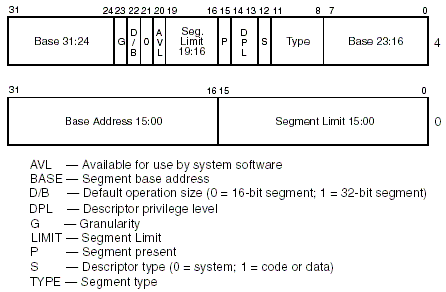
\includegraphics[width=9cm]{imagenes/gdt.png}
\end{center}
\end{figure}

En éste ejercicio vamos a definir 4 segmentos, cada uno con su entrada en la GDT.

\subparagraph*{Entrada 1}
\begin{itemize}
	
    \item $.base_{0-15}$ = 0,

    \item $.base_{23-16}$ = 0,
    \item $.base_{31-24}$ = 0,
    
El segmento empieza en la dirección de memoria 0.
        
    \item $.limit_{0-15}$ = 0xDCFF,
    \item $.limit_{16-19}$ = 0x2;

733 MB = 187648 bloques de 4 KB.
\\ El máximo offset que queremos utilizar es 187648 - 1 = 0x2DCFF 
    
    \item .type = 8
        
Será un segmento de código $Execute-Only$.
        
    \item .s  = 1
        
Código/Datos \fixme{explicar que significa esto}
        
    \item .dpl = 0
        
Este segmento tendrá nivel de privilegio 0.

    \item .p = 1
        
Este segmento estará presente en memoria.  \fixme{asi se expresa?}
    
    \item .avl = 0
        
A disposición del programador.


    \item .l = 0
        
Sólo va en 1 cuando estás en modo IA-32e \fixme{no esta en nuestro dibujo}

    \item .db = 1
        
Siginifica que vamos a trabajar en 32 bits. \fixme{especificamente?}

    \item .g = 1

Nuestro límite lo vamos a expresar con una granularidad de 4KB en vez de 1B. Es decir, vamos a poder direccionar (limite - 1) * 4K bytes.

\end{itemize}

\subparagraph*{Entrada 2}

Se diferencia de la entrada 1 en que el campo $dpl$ - el nivel de privilegio - se pone en 3.

\subparagraph*{Entrada 3}

Se diferencia de la entrada 1 en que el campo $type$ se pone en 2 - $Read-Write$.

\subparagraph*{Entrada 4}

Se diferencia de la entrada 3 en que el campo $dpl$ se pone en 3.




% Ejercicio 1 - b)
\paragraph{Modo Protegido}\label{subsubsec:ej1-b}
Completar el código necesario para pasar a modo protegido y setear la pila del
kernel en la dirección 0x27000.
\hruler

Primero cargamos la GDT, pasandole su descriptor como parámetro a la instrucción LGDT. Deshabilitamos las interrupciones y seteamos el bit PE del
registro $CR0$ en 1. \fixme{para que?}
Habilitamos el el pin A20 para poder acceder a direcciones de memoria superiores al MB.
En éste momento se hace un $FAR$ $JUMP$ hacia la siguiente instrucción, utilizando como selector de segmento el offset en la GDT de la primer 
entrada definida más arriba (de código de nivel de administrador).
Se procede a cargar los selectores de segmento y setear la base de la pila.

% Ejercicio 1 - c)
\paragraph{GDT - Área de Memoria}\label{subsubsec:ej1-c}
Declarar un segmento adicional que describa el área de la pantalla en memoria
que pueda ser utilizado sólo por el kernel.
\hruler

En la GDT ya habíamos definido una quinta entrada para el segmento de la memoria de video.

Tiene la base en la posición 0xB8000. Como sólo va a direccionar \fixme{}

% Ejercicio 1 - d)
\paragraph{Limpiar la pantalla}\label{subsubsec:ej1-d}
Escribir una rutina que se encargue de limpiar la pantalla y pintar el area de
el mapa un fondo de color (sugerido verde). Para este ejercicio se debe escribir
en la pantalla usando el segmento declarado en el punto anterior (para los
próximos ejercicios se accederá a la memoria de vídeo por medio del segmento de
datos de 773MB).

Nota: La GDT es un arreglo de gdt entry declarado sólo una vez como gdt. El
descriptor de la GDT en el código se llama GDT DESC.

\hruler
La pantalla en este caso es una matriz en donde cada posición es un caracter ASCII con un determinado color de letra y fondo. La rutina es un
simple ciclo que va escribiendo el caracter nulo con un fondo verde sobre las posiciones de (0, 0) a (50, 50), que representan el campo de
batalla.

  \clearpage

  % -- Ejercicio 2 --
  \subsection{Ejercicio 2}\label{subsec:ej2}
  %\setcounter{paragraph}{1}
% Ejercicio 2 - a)
\paragraph{}\label{subsubsec:ej2-a}
Completar las entradas necesarias en la IDT para asociar diferentes rutinas a
todas las excepciones del procesador. Cada rutina de excepción debe indicar en
pantalla qué problema se produjo e interrumpir la ejecución. Posteriormente se
modificarán estas rutinas para que se continúe la ejecución, resolviendo el
problema y desalojando a la tarea que lo produjo.
\hruler
\fixme{Respuesta}

La IDT - $Interrupt$ $Descriptor$ $Table$ - es una tabla de descriptores de manejadores de interrupción. Cada entrada describe la atención de
un tipo de interrupción en particular. Tiene la siguiente forma:

\begin{figure}[H]
\begin{center}
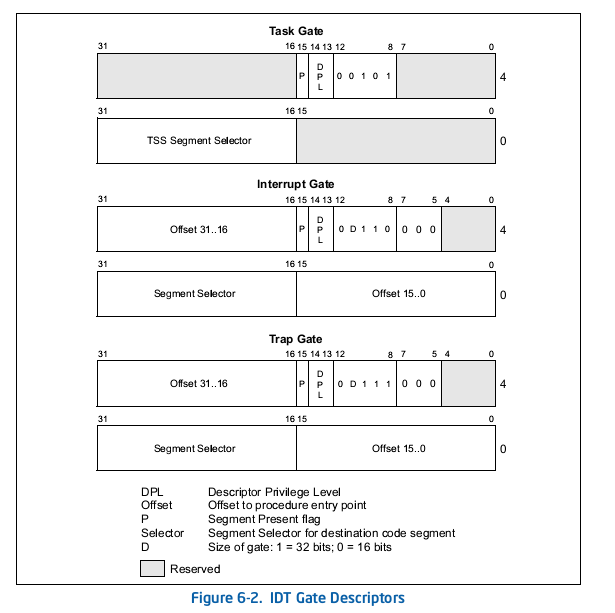
\includegraphics[]{imagenes/idt_entry.png}
\end{center}
\end{figure}

\fixme{decidir si lo que queremos es int, trap, gate}

En éste ejercicio vamos a ocuparnos de las excepciones del procesador, cuyo tipo va entre 0 y 19.
Para cada una nuestra rutina de atención será imprimir los detalles de la excepción, según el manual de Intel. \fixme{y autodestruirse?}
Con tal propósito llenamos las entradas de la IDT de la siguiente forma.

\begin{itemize}
    \item segment-selector = 0x40 (de código de nivel 0)
    \item offset = la dirección donde escribimos la rutina de tal excepción
    \item p = 1 (presente)
    \item dpl = 0 (nivel administrador)
    \item d = \fixme{?}
\end{itemize}

% Ejercicio 2 - b)
\paragraph{}\label{subsubsec:ej2-b}
Hacer lo necesario para que el procesador utilice la IDT creada anteriormente.
Generar una excepción para probarla.

Nota: La IDT es un arreglo de idt entry declarado solo una vez como idt. El
descriptor de la IDT en el código se llama IDT DESC. Para inicializar la IDT se
debe invocar la función idt inicializar.
\hruler
\fixme{la que hiciste vos Eze}

  \clearpage

  % -- Ejercicio 3 --
  \subsection{Ejercicio 3}\label{subsec:ej3}
  % Ejercicio 3 - a)
\paragraph{replace-me-with-a-descriptive-text}\label{subsubsec:ej3-a}
Escribir una rutina que se encargue de limpiar el buffer de vídeo y pintarlo
como indica la figura 8. Tener en cuenta que deben ser escritos de forma
genérica para posteriormente ser completados con información del sistema. Además
considerar estas imágenes como sugerencias, ya que pueden ser modificadas a
gusto según cada grupo mostrando siempre la misma información.
\hruler
\fixme{Respuesta}

% Ejercicio 3 - b)
\paragraph{replace-me-with-a-descriptive-text}\label{subsubsec:ej3-b}
Escribir las rutinas encargadas de inicializar el directorio y tablas de páginas
para el kernel (mmu inicializar dir kernel). Se debe generar un directorio de
páginas que mapee, usando identity mapping, las direcciones 0x00000000 a
0x00DC3FFF, como ilustra la figura 5. Además, esta función debe inicializar el
directorio de páginas en la dirección 0x27000 y las tablas de páginas según
muestra la figura 1.
\hruler
\fixme{Respuesta}
bit ti = 0, significa que lo va a buscar a la gdt

% Ejercicio 3 - c)
\paragraph{replace-me-with-a-descriptive-text}\label{subsubsec:ej3-c}
Completar el código necesario para activar paginación.
\hruler
\fixme{Respuesta}

% Ejercicio 3 - d)
\paragraph{replace-me-with-a-descriptive-text}\label{subsubsec:ej3-d}
Escribir una rutina que imprima el nombre del grupo en pantalla. Debe estar
ubicado en la primer linea de la pantalla alineado a derecha.
\hruler
\fixme{Respuesta}

  \clearpage

  % -- Ejercicio 4 --
  \subsection{Ejercicio 4}\label{subsec:ej4}
  % Ejercicio 4 - a)
\paragraph{replace-me-with-a-descriptive-text}\label{subsubsec:ej4-a}
Escribir una rutina (inicializar mmu) que se encargue de inicializar las
estructuras necesarias para administrar la memoria en el area libre.
\hruler
\fixme{Respuesta}

% Ejercicio 4 - b)
\paragraph{replace-me-with-a-descriptive-text}\label{subsubsec:ej4-b}
Escribir una rutina (mmu inicializar dir tarea) encargada de inicializar un
directorio de páginas y tablas de páginas para una tarea, respetando la figura
5. La rutina debe copiar el código de la tarea a su área asignada, es decir sus
dos páginas de código dentro de el mapa y mapear dichas páginas a partir de la
dirección virtual 0x08000000(128MB).
\hruler
\fixme{Respuesta}

% Ejercicio 4 - c)
\paragraph{replace-me-with-a-descriptive-text}\label{subsubsec:ej4-c}
Escribir dos rutinas encargadas de mapear y desmapear páginas de memoria.

I- mmu mapear pagina(unsigned int virtual, unsigned int cr3, unsigned int
fisica) Permite mapear la página física correspondiente a fisica en la dirección
virtual virtual utilizando cr3.

II- mmu unmapear pagina(unsigned int virtual, unsigned int cr3). Borra el mapeo
creado en la dirección virtual virtual utilizando cr3.
\hruler
\fixme{Respuesta}

% Ejercicio 4 - d)
\paragraph{replace-me-with-a-descriptive-text}\label{subsubsec:ej4-d}
Construir un mapa de memoria para tareas e intercambiarlo con el del kernel,
luego cambiar el color del fondo del primer caracter de la pantalla y volver a
la normalidad.

Nota: Por la construcción del kernel, las direcciones de los los mapas de
memoria (page directory y page table) están mapeadas con identity mapping. En
los ejercicios en donde se modifica el directorio o tabla de páginas, hay que
llamar a la función tlbflush para que se invalide la cache de traducción de
direcciones.
\hruler
\fixme{Respuesta}

  \clearpage

  % -- Ejercicio 5 --
  \subsection{Ejercicio 5}\label{subsec:ej5}
  % Ejercicio 5 - a)
\paragraph{replace-me-with-a-descriptive-text}\label{subsubsec:ej5-a}
Completar las entradas necesarias en la IDT para asociar una rutina a la
interrupción del reloj, otra a la interrupción de teclado y por último una a la
interrupción de software 0x52.
\hruler
\fixme{Respuesta}

% Ejercicio 5 - b)
\paragraph{replace-me-with-a-descriptive-text}\label{subsubsec:ej5-b}
Escribir la rutina asociada a la interrupción del reloj, para que por cada tick
llame a la función screen proximo reloj. La misma se encarga de mostrar cada vez
que se llame, la animación de un cursor rotando en la esquina inferior derecha
de la pantalla. La función proximo reloj está definida en isr.asm.
\hruler
\fixme{Respuesta}

% Ejercicio 5 - c)
\paragraph{replace-me-with-a-descriptive-text}\label{subsubsec:ej5-c}
Escribir la rutina asociada a la interrupción de teclado de forma que si se
presiona cualquier número, se presente el mismo en la esquina superior derecha
de la pantalla. El número debe ser escrito en color blanco con fondo de color
aleatorio por cada tecla que sea presionada\footnote{http://wiki.osdev.org/Text
UI}.
\hruler
\fixme{Respuesta}

% Ejercicio 5 - d)
\paragraph{replace-me-with-a-descriptive-text}\label{subsubsec:ej5-d}
Escribir la rutina asociada a la interrupción 0x52 para que modifique el valor
de eax por 0x42. Posteriormente este comportamiento va a ser modificado para
atender los servicios del sistema.
\hruler
\fixme{Respuesta}

  \clearpage

  % -- Ejercicio 6 --
  \subsection{Ejercicio 6}\label{subsec:ej6}
  % Ejercicio 6 - a)
\paragraph{replace-me-with-a-descriptive-text}\label{subsubsec:ej6-a}
Definir 3 entradas en la GDT para ser usadas como descriptores de TSS. Una será
reservada para la tarea inicial y otras dos para realizar el intercambio entre
tareas, denominadas TSS1 y TSS2 respectivamente.
\hruler
\fixme{Respuesta}

% Ejercicio 6 - b)
\paragraph{replace-me-with-a-descriptive-text}\label{subsubsec:ej6-b}
Completar la entrada de la TSS1 con la información de la tarea Idle. Esta
información se encuentra en el archivo TSS.C. La tarea Idle se encuentra en la
dirección 0x00020000. La pila se alojará en la misma dirección que la pila del
kernel y será mapeada con identity mapping. Esta tarea ocupa 2 paginas de 4KB y
debe ser mapeada con identity mapping. Además la misma debe compartir el mismo
CR3 que el kernel.
\hruler
\fixme{Respuesta}

% Ejercicio 6 - c)
\paragraph{replace-me-with-a-descriptive-text}\label{subsubsec:ej6-c}
Completar el resto de la información correspondiente a cada tarea en la
estructura auxiliar de contextos. El código de las tareas se encuentra a partir
de la dirección 0x00010000 ocupando dos páginas de 4kb cada una. El mismo debe
ser mapeado a partir de la dirección 0x08000000. Para la dirección de la pila se
debe utilizar el mismo espacio de la tarea, la misma crecerá desde la base de la
tarea. Para el mapa de memoria se debe construir uno nuevo para cada tarea
utilizando la función mmu inicializar dir usuario. Además, tener en cuenta que
cada tarea utilizará una pila distinta de nivel 0, para esto se debe pedir una
nueva pagina libre a tal fin.
\hruler
\fixme{Respuesta}

% Ejercicio 6 - d)
\paragraph{replace-me-with-a-descriptive-text}\label{subsubsec:ej6-d}
Completar la entrada de la GDT correspondiente a la tarea inicial.
\hruler
\fixme{Respuesta}

% Ejercicio 6 - e)
\paragraph{replace-me-with-a-descriptive-text}\label{subsubsec:ej6-e}
Completar la entrada de la GDT correspondiente a la TSS1, que contiene la
información de la tarea Idle.
\hruler
\fixme{Respuesta}

% Ejercicio 6 - f)
\paragraph{replace-me-with-a-descriptive-text}\label{subsubsec:ej6-f}
Completar la entrada de la GDT correspondiente a la TSS2.
\hruler
\fixme{Respuesta}

% Ejercicio 6 - g)
\paragraph{replace-me-with-a-descriptive-text}\label{subsubsec:ej6-g}
Escribir el código necesario para ejecutar la tarea Idle, es decir, saltar
intercambiando las TSS, entre la tarea inicial y la tarea Idle.

Nota: En tss.c están definidas las tss como estructuras TSS. Trabajar en tss.c y
kernel.asm.
\hruler
\fixme{Respuesta}

  \clearpage

  % -- Ejercicio 7 --
  \subsection{Ejercicio 7}\label{subsec:ej7}
  % Ejercicio 7 - a)
\paragraph{replace-me-with-a-descriptive-text}\label{subsubsec:ej7-a}
Construir una función para inicializar las estructuras de datos del scheduler.
\hruler
\fixme{Respuesta}

% Ejercicio 7 - b)
\paragraph{replace-me-with-a-descriptive-text}\label{subsubsec:ej7-b}
Crear la función sched proximo indice() que devuelve el índice en la GDT de la
próxima tarea a ser ejecutada. Construir la rutina de forma devuelva el indice
de la TSS1 y luego el de la TSS2 de forma intercalada, para dos tareas fijas.
\hruler
\fixme{Respuesta}

% Ejercicio 7 - c)
\paragraph{replace-me-with-a-descriptive-text}\label{subsubsec:ej7-c}
Modificar la rutina de la interrupción 0x52, para que implemente los tres
servicios del sistema según se indica en la sección 3.1.1.
\hruler
\fixme{Respuesta}

% Ejercicio 7 - d)
\paragraph{replace-me-with-a-descriptive-text}\label{subsubsec:ej7-d}
Modificar el código necesario para que se realice el intercambio de tareas por
cada ciclo de reloj. El intercambio se realizará según indique la función sched
proximo indice().
\hruler
\fixme{Respuesta}

% Ejercicio 7 - e)
\paragraph{replace-me-with-a-descriptive-text}\label{subsubsec:ej7-e}
Modificar la función sched proximo indice() de forma que ejecute todas las
tareas según se describe en la sección 3.2.
\hruler
\fixme{Respuesta}

% Ejercicio 7 - f)
\paragraph{replace-me-with-a-descriptive-text}\label{subsubsec:ej7-f}
Modificar las rutinas de excepciones del procesador para que impriman el
problema que se produjo en pantalla, desalojen a la tarea que estaba corriendo y
corran la próxima, indicando en pantalla porque razón fue desalojada la tarea en
cuestión. Nota: Se recomienda construir funciones en C que ayuden a resolver
problemas como convertir direcciones de el mapa a direcciones físicas.
\hruler
\fixme{Respuesta}

  \clearpage

  % -- Ejercicio 8 --
  \subsection{Ejercicio 8 (optativo)}\label{subsec:ej8}
  % Ejercicio 8 - a)
\paragraph{replace-me-with-a-descriptive-text}\label{subsubsec:ej8-a}
Crear un tanque (tarea) propio que mapee paginas a muerte contra otros
intrepidos tanques. Para esto pueden editar el código del primer tanque a gusto.
El tanque debe tener las siguientes características,

\begin{itemize}
  \item No ocupar más de 8 kb (tener en cuenta la pila).
  \item Tener como punto de entrada la dirección cero.
  \item Estar compilada para correr desde la dirección 0x08000000.
  \item Utilizar solo los servicios presentados en el trabajo práctico.
\end{itemize}

Explicar en pocas palabras qué estrategia utilizaron en su tanque en términos de
<<defensa>> y <<ataque>>.
\hruler
\fixme{Respuesta}

% Ejercicio 8 - b)
\paragraph{replace-me-with-a-descriptive-text}\label{subsubsec:ej8-b}
Si consideran que su tanque es capaz de enfrentarse contra los tanques del
resto de sus compañeros, pueden enviar el binario a la lista de docentes
indicando los siguientes datos,

\begin{itemize}
  \item Nombre del tanque, ej: \emph{T-90S Bhishma}
  \item Características letales, ej: \emph{Cañón 2A46M de 125 mm con cargador 
    automático}
  \item Sistema de defensa, ej: \emph{1.350 mm en blindaje laminado, blindaje 
    reactivo...}
\end{itemize}

Se realizará una competencia a fin de cuatrimestre con premios en/de chocolate
para los primeros puestos.
\hruler
\fixme{Respuesta}

% Ejercicio 8 - c)
\paragraph{replace-me-with-a-descriptive-text}\label{subsubsec:ej8-c}
Mencionar la mayor cantidad de características del tanque montado en el jardín
del edificio Libertador en la ciudad de Buenos Aires.
\hruler
\fixme{Respuesta}

  \clearpage

\end{document}